%======================================================================
\chapter{Implementation}
\label{ch: implementation}
%======================================================================

Since this project was a new concept, the implementation had to start from scratch. Although there have been projects in the past that have used XBees to get signal strength, none of them used it in the same way as this project. For this project a mobile robot and a remote first had to be built to use for testing. Then a code base needed to be created to control the mobile robot according to the design algorithms.

%----------------------------------------------------------------------
\section{Robot Assembly}
\label{sec:Robot Assembly}
%----------------------------------------------------------------------

For this project, a Remote Target and Smart Robotic Cart were designed and implemented from off-the-shelf components.  As mentioned above in section \ref{sec:System Components}, some of the components were already available at Bradley University, and others had to be purchased specifically for this project. The parts are listed in \autoref{tab:Partslablist} and \autoref{tab:Partslist}.

\vspace*{12pt}
\noindent
Since the school already owned the Budget Bot chassis, it was a good choice for the base of the  Smart Robotic Cart. However, the Budget Bot chassis was modified slightly to work for this project. The main change was swapping out the motors that came with the Budget Bot for Pololu 27D Metal Gear motors since the original motors have a max speed of 212 RPM or 1.09m/s and the new motors have a max speed of 530 RPM or 2.72m/s when using the wheels with a diameter of 98mm. By switching out the motors enabled the robot to move faster to make it better able to achieve the goal of matching an average person's walking speed. The other modifications to the chassis were a hard power switch to directly cut off power to the XBee modules in the reflector and a power LED to indicate when this switch was on.

\vspace*{12pt}
\noindent
The next step was to attach the BeagleBone Blue microcomputer, XBee reflector array assembly, and breadboard to the top of the robot. A 2-cell LiPo battery was also installed inside the chassis of the mobile cart to provide power to the BeagleBone Blue directly and the breadboard through the switch. The power supplied to the breadboard is sent through a regulator circuit to drop it down from the 7.4V of the LiPo to 3.3V of the XBee. This circuit is also used on the remote which consists of a 7.4V LiPo battery and the XBee module with voltage regulator in between. This voltage regulator is built out of a LM117 regulator and a 10uF ceramic capacitor between the input and output pins of the regulator. The circuit diagrams for the robot and remote are shown in Figs. \ref{fig:robotCircuit} and \ref{fig:remoteCircuit}.
\begin{figure}[H]
    \centering
    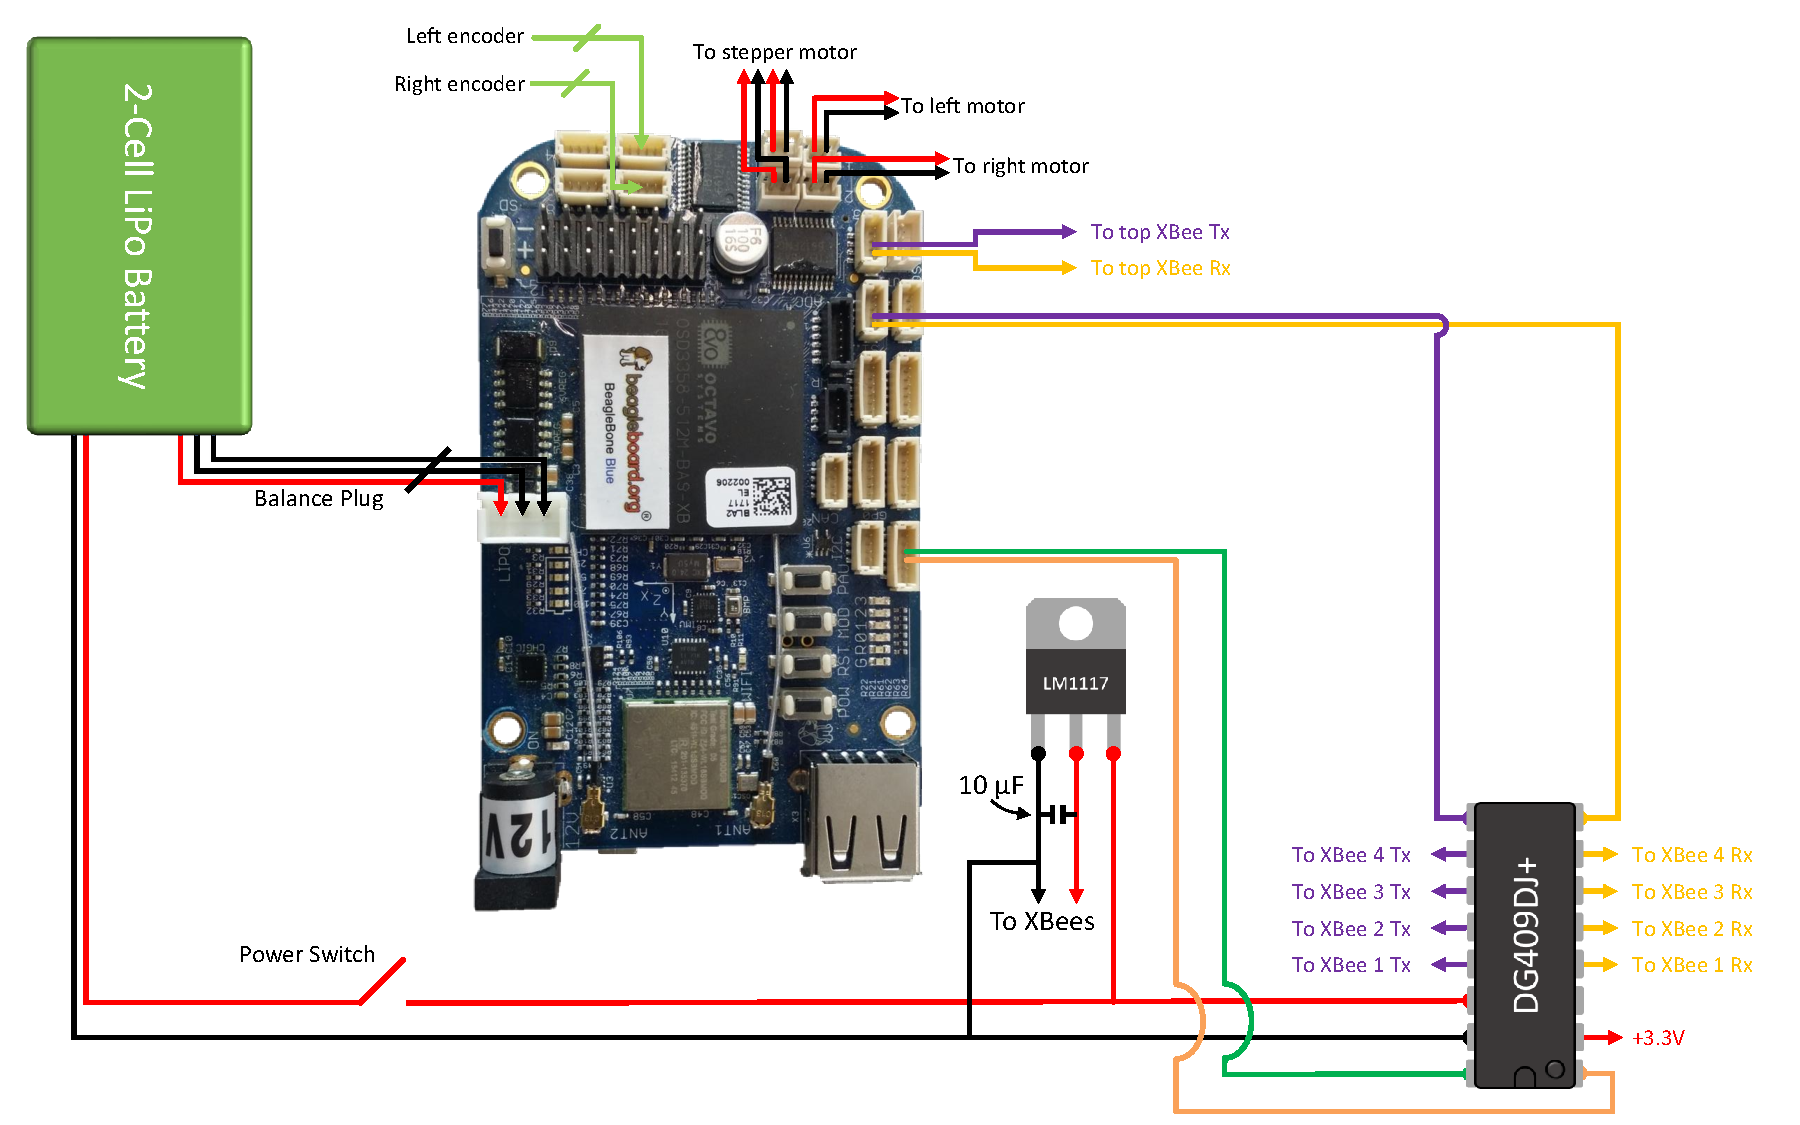
\includegraphics[width=\textwidth]{figs/robotCircuit.pdf}
    \caption{Circuit Diagram for Robotic Cart}
    \label{fig:robotCircuit}
\end{figure}
\begin{figure}[H]
    \centering
    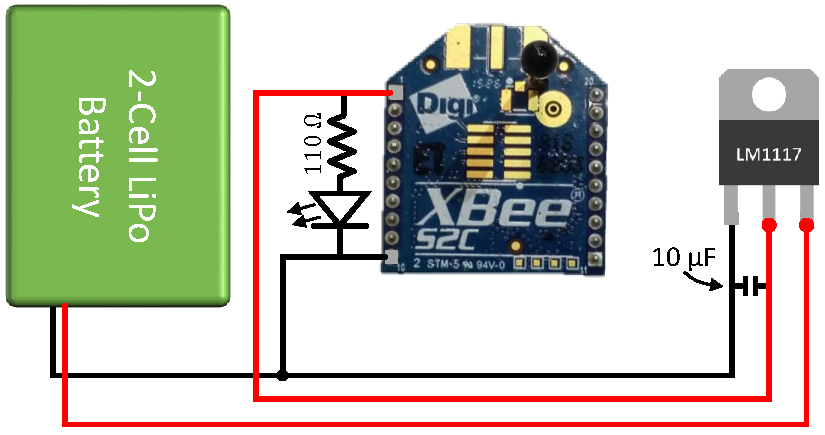
\includegraphics[width=0.7\textwidth]{figs/remoteCircuit.pdf}
    \caption{Circuit Diagram for Remote}
    \label{fig:remoteCircuit}
\end{figure}

\vspace*{12pt}
\noindent
The reflector array assembly from \autoref{sec:customReflector} was mounted on a stepper motor that was then attached to a 3D printed bracket. This bracket was then attached to the chassis using M3 screws. Another feature of this bracket is that it had a stop block built into the top  to allow the robot to automatically initialize the reflector array to the zero position when the robot starts up. This is accomplished by commanding a turn of 90\textdegree and allowing the reflectors to hit the stop block and be held there until this turn is complete.

\vspace*{12pt}
\noindent
The Xbee modules from the reflector array posed a bit of a problem when it came to connecting them to the BeagleBone Blue. The BeagleBone Blue has three standard UART ports and two others found in the USB and UART-GPS, which makes a total of five UARTs. Unfortunately not all five ports can be used to communicate with XBees since UART0 is used to provide communication with a computer through the console. Since port 0 is reserved for this function, the number of usable ports is only four, but the project requires communication with five XBees. The solution to this problem was to use two of the GPIO pins, two of the UART ports, and a dual 4-channel multiplexer. One of the UARTs can be directly connected to the top XBee, and the other UART can be routed through the multiplexer to the four side XBee modules. Then two UART ports are used to communicate with all five XBees.

\vspace*{12pt}
\noindent
Instructions for assembling the robot can be found in \autoref{ch: assemblyInstructions}. Therein, the sequence of steps is explained in detail with pictures to show the state of the robot. The finished prototype robot and remote are shown in Fig. \ref{fig:finishedPrototypes}.

\begin{figure}[H]
    \centering
    \begin{subfigure}[t]{0.5\textwidth}
        \centering
        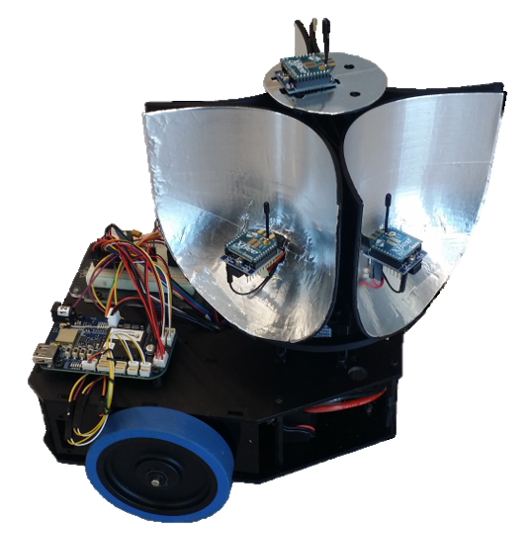
\includegraphics[width=\textwidth]{figs/img/Finalized_robot.png}
        \captionsetup{width=\textwidth}
        \caption{Robotic Cart Prototype}
        \label{fig:overallPrototype}
    \end{subfigure}
    \begin{subfigure}[t]{0.35\textwidth}
        \centering
        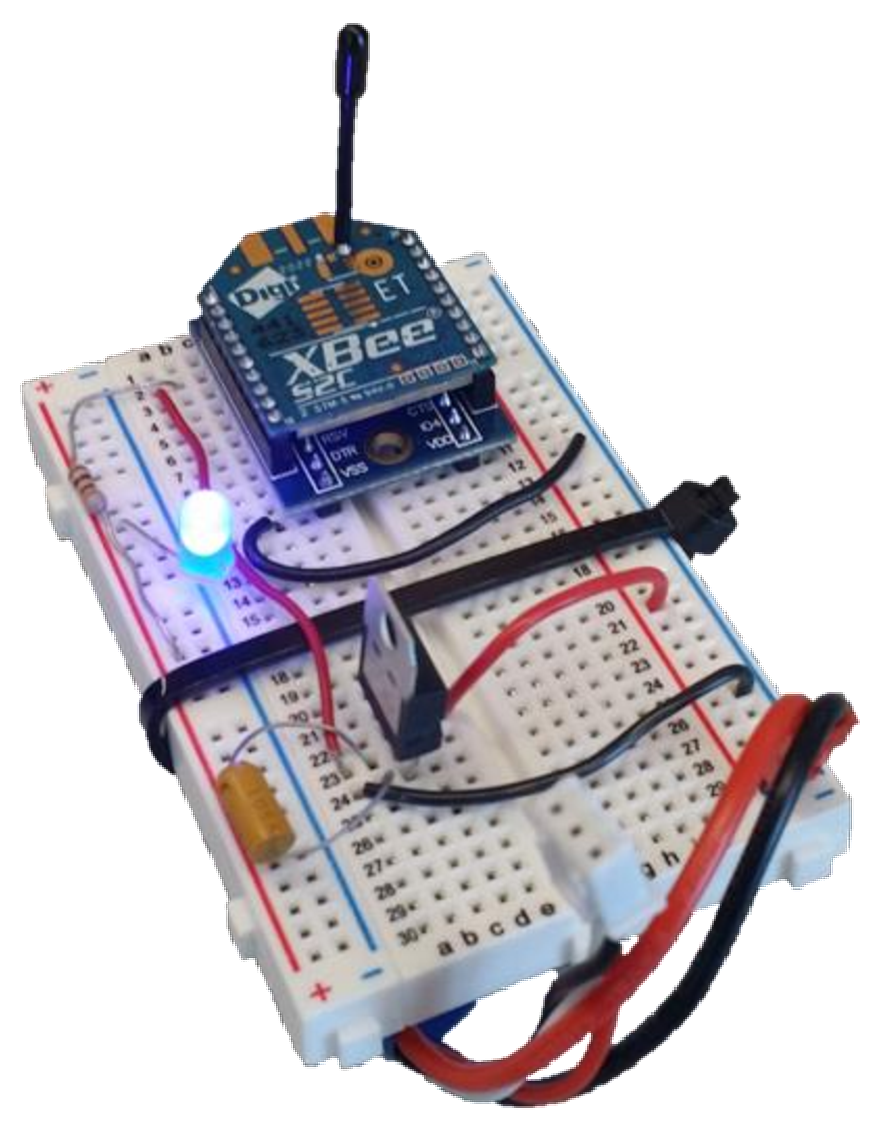
\includegraphics[width=\textwidth]{figs/remote.pdf}
        \captionsetup{width=\textwidth}
        \caption{Remote Prototype}
        \label{fig:remotePrototype}
    \end{subfigure}
    \caption{Finished Prototypes}
    \label{fig:finishedPrototypes}
\end{figure}


%----------------------------------------------------------------------
\section{Code Base}
\label{sec:Code Base}
%----------------------------------------------------------------------

For the project some base functionality was needed to use with the main follower program so it could interact with the other components in the system. The BeagleBone Blue already has a set of ports on it that can be accessed and controlled using the Robot Control Library from Strawson Design ~\cite{Robot_Control_Library}.

\vspace*{12pt}
\noindent
Some custom libraries were built on top of the Robot Control Library to handle XBee Frames, AT Commands, and the stepper motor control. The XBee Frames library takes a given block of data containing the message and then packages it into a XBee Frame to send over UART to the XBee desired module. The XBee communications library also handles received messages from the XBee module and validates the received frame's integrity and extracts the message data from it. On top of the XBee communications library there is a library that generates AT Commands to package in the XBee Frames. The AT Command library also handles extracting response data from the AT Response Command structure and validates it.

\begin{figure}[H]
  \centering
  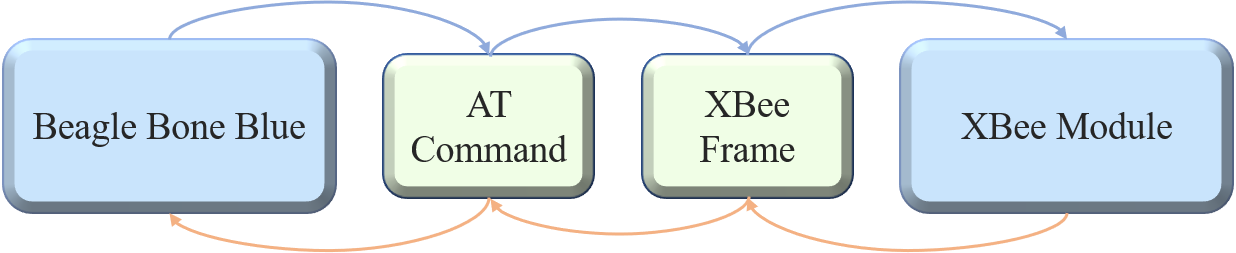
\includegraphics[width=\textwidth]{figs/img/Command Process Diagram.png}
  \caption{Process for XBee Communication over UART}
  \label{fig:CommandProcessDiagram}
\end{figure}

\vspace*{12pt}
\noindent
The final custom library is the stepper motor control library. This library had to be written since instead of using a dedicated stepper motor controller, two of the regular BBBlue DC motor control ports were used to power the stepper motor. The library handled translating how many steps to turn into the phase states to be sent to the DC motor ports that are connected to the stepper motor. The library also helped to keep track of basic information related to the stepper motor such as what its current angle should be.

%----------------------------------------------------------------------
\section{Experimental Results}
\label{sec:Experimental Results}
%----------------------------------------------------------------------

After the Robotic Cart, Remote Target, and code base were built, several different variants of the algorithms explained in \autoref{sec:locAndNavAlgos} were tested. There were two main types of variants tested. In one variant, the stepper motor is locked, preventing the reflector from rotating. In the other variant, the stepper motor is used to sweep through the angles.

\subsection{Rotating Reflector Tests}

The first type of test was where the robot would initialize the reflector array to the zero point with the stepper motor, then rotate in nine degree increments taking measurements as it went. A sweep ends when the motor has turned 81 degrees since at that point, with the four sides of the reflector, a full 360 degrees has been scanned.

\vspace*{12pt}
\noindent
This method offers a sufficiently dense set of data to base the angle predictions off of, but at the cost of having to wait until a entire sweep of the reflectors is completed for a single estimation of the remote location. The first attempt with this method was a simple test that would continuously sweep the reflectors and move the robot at the same time. Though this version did eventually make its way toward the remote, it had some errors in the robot's navigation trajectory. For example, the robot would correctly turn towards the remote, however, if it picked up a stronger signal from the XBee reverberations, it would drive off in a different direction. The robot would eventually find its way back into alignment and resume moving towards the remote.

\vspace*{12pt}
\noindent
The next version that used a rotating reflector, as well as the final version, works mostly the same as the first version, but with some improvements to the navigation. It was determined that the oscillations in the robot's trajectory in the first test were a result of turning the robot while also rotating the reflector. This adds additional rotation to the measurements in the global scope. Due to the design of the robot, the reflector array can only be rotated 90 degrees, but to properly fix this rotation issue the reflector array would need to be rotated more or less during a sweep to compensate for the robot's rotation. The solution was simply to alternate between sweeping the reflector and rotating the robot, all the while allowing the robot to always move forward. The rotation of the robot was limited to 15\textdegree before another measurement would be taken. In this version some additional windowed filters to average out the angle measurements were added, which did help to reduce the effects of random angles from noise in the system. Based on data collected in an anechoic chamber, offsetsfor each of the directional receivers were applied to try to convert the received signal strengths to use the same baseline. This offset was needed since each XBee would receive slightly different signal strengths when it was pointed directly at the remote.

\subsection{Locked Reflector Tests}

The locked reflector tests were run in between the first algorithm and the final algorithm which ultimately used a sweeping function to capture the XBee signals. The locked reflector algorithms were an attempt to reduce the time needed to get a set of measurements from the reflector by zeroing its rotation and then keeping it locked in the zero position. Since the data from this is relatively sparse, three different methods for estimating the angle of the remote were attempted. The first of these three methods was to try to select the direction that the signal was coming strongest from and then which of its two neighbor directions had the second strongest signal. With these two strengths the algorithm would then try to interpolate the angle based on the difference of the strengths between them. This method could possibly work, but due to the time constraints of the project, there was not enough time to implement and test this method.

\vspace*{12pt}
\noindent
The other two methods that were tried with the locked reflector were both different variants on machine learning algorithms. A small pool of data was collected both in an anechoic chamber and in a normal operating environment. The first algorithm attempted to use the K Nearest Neighbors algorithm to estimate the angle of the remote based on the relative signal strengths received by the directional XBees. The second algorithm used a neural network to predict the angle. Both of these algorithms failed to produce meaningful results, probably due to the fact that there was a very small pool of data to work with compared to the large amounts of data needed to perform machine learning algorithms. The noise in the signals proved too much for these algorithms to handle elegantly. If data were collected in many operating environments, machine learning techniques may be able to yield favorable results.

\subsection{System noise}

In both the fixed and sweeping experiments, an underlying issue was the amount of noise in the system. The first type of noise that occurs is noise from the multipath effect, where the signals bounce off obstacles in the environment, adding constructing and destructive interference randomly based on the robot's surroundings. The second source of noise was internal noise in the XBees, which was worse than what was expected. The XBee internal noise was isolated using an anechoic chamber where all the signals strengths did become stronger, but the base noise from the XBees persisted. The noise coming from the XBees tends to be about 2 to 6 dBm on average. The change from facing towards the remote then away from the remote is about 13 to 15 dBm. These ranges result in the occasional measurement that flip flops which reflector is actually facing the remote. The noise can be seen in the test measurements that were collected where 300 measurements were taken at several intervals around the robot as seen in Fig. \ref{fig:SensorDataGraphs}.

\begin{figure}[H]
    \centering
    \begin{subfigure}{0.50\textwidth}
        \centering
        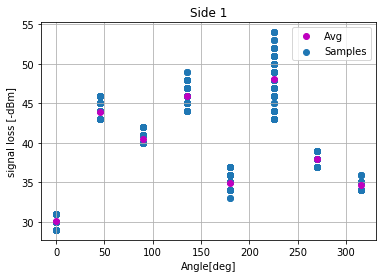
\includegraphics[width=0.95\textwidth]{figs/img/Side1_Data.png}
        \label{fig:Side1Dat}
    \end{subfigure}%
    \begin{subfigure}{0.50\textwidth}
        \centering
        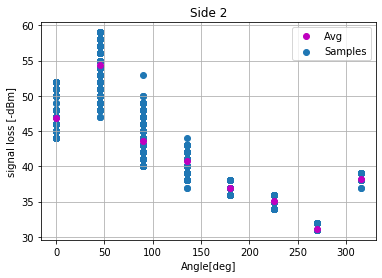
\includegraphics[width=0.95\textwidth]{figs/img/Side2_Data.png}
        \label{fig:Side2Dat}
    \end{subfigure}
        \begin{subfigure}{0.50\textwidth}
        \centering
        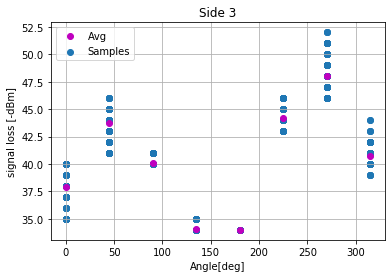
\includegraphics[width=0.95\textwidth]{figs/img/Side3_Data.png}
        \label{fig:Side3Dat}
    \end{subfigure}%
    \begin{subfigure}{0.50\textwidth}
        \centering
        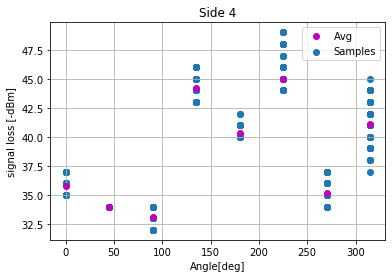
\includegraphics[width=0.95\textwidth]{figs/img/Side4_Data.png}
        \label{fig:Side4Dat}
    \end{subfigure}
    \caption{Navigation Algorithm Details}
    \label{fig:SensorDataGraphs}
\end{figure}

\subsection{Distance}
This project initially planned to use the top XBee module's signal strength to determine the distance to the remote. In practice, however, it was determined to be nearly impossible with the current setup. The free-space path loss equation was used as a base equation to attempt to implement this feature in the project. One problem is that the free-space path loss formula is for use in free space, so it fails to yield the correct distance whenever any form of obstacle ends up in the line-of-sight path to the remote. The free-space path loss formula is also thrown off by any reflective surfaces around it due to the multipath effect. These issues could be potentially solved using a simultaneous localization and mapping algorithm such as EKF-SLAM.  Unfortunately, this approach would be very difficult since it relies on a known global reference point, but the robot in this project has no such global reference. It was decided that the distance measurement would be put on hold for future work on this project.

\section{Simulation using Robot Simulator}

Before constructing the physical robot prototype, a simulation was performed using a commercial robot simulator, CoppeliaSim. However, since RF signal behavior depends highly on the environment, the system could not be fully simulated. This section explains the steps taken to simulate the proposed robotic cart.

\vspace*{12pt}
\noindent
First, a model of the Budget Bot chassis was created in CoppeliaSim. The model is shown in Fig. \ref{fig:budgetBotModel}. The model was designed with the same dimensions as the physical chassis to accurately simulate the robot kinematics. Details on modeling a robot chassis in CoppeliaSim can be found in \autoref{ch: coppSimModeling}. Although \autoref{ch: coppSimModeling} explains the modeling of a robot chassis that is different than the Budget Bot chassis, the concepts are the same for modeling any robot chassis.
\begin{figure}[H]
    \centering
    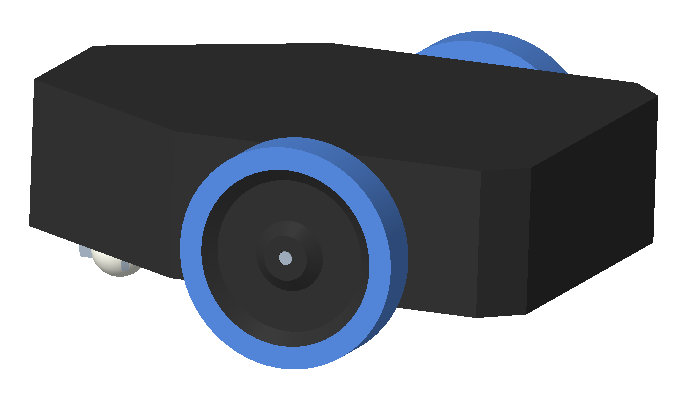
\includegraphics[width=0.4\textwidth]{figs/img/budgetBotModel.png}
    \caption{Model of Budget Bot Chassis}
    \label{fig:budgetBotModel}
\end{figure}

\noindent
MATLAB code was written to control the simulation. The actual distance between the robot and the remote was measured, then random noise was added with a mean of 0 and a standard deviation of 0.07. This noisy measurement was then used in the navigation algorithm to determine how to drive the robot (see \autoref{subsec:navAlgo}). An image of the simulation is shown in Fig. \ref{fig:coppSimExample}, where the blue sphere represents the remote, and the green dot represents the target point.
\begin{figure}[H]
    \centering
    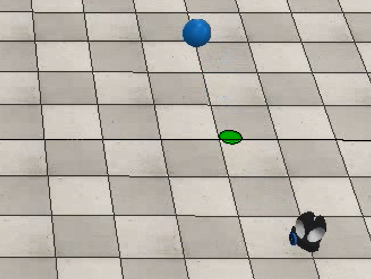
\includegraphics[width=0.5\textwidth]{figs/img/coppSimExample.png}
    \caption{CoppeliaSim Simulation}
    \label{fig:coppSimExample}
\end{figure}


%%% Local Variables:
%%% mode: latex
%%% TeX-master: "../finalReport"
%%% End:
